%
%
% jc-draft_2_method.tex
%
%
%
\documentclass[jctc-draft.tex]{subfiles}
\begin{document}
\section{Method}
\label{sec:method}
In this section, we first outline the configuration of the simulator circuit
evaluated in this study and the hydrogen atom models targeted for simulation .
Subsequently, we detail the specific methodologies for the three main challenges
addressed in this paper: (1) a circuit configuration executable on an emulator,
(2) the handling of the singularity (pole) of the Coulomb potential, and (3) a
method for determining simulation parameters that minimize errors.

\subsection{Overview of the Simulator and Computational Model}
\label{subsec:simulator-model}
In this study, simulator circuits are generated using Chemical Reaction
Simulator Q (crsQ) \cite{website:crsq}, a quantum chemistry simulator software
for quantum computers developed by the authors. crsQ features the ability to
generate quantum circuits for a wide range of configurations according to the
target model and simulation conditions. The models addressed in this paper are
single hydrogen atom models, where the nucleus is treated as stationary at the
origin of the coordinate system. We consider spatial dimensions of 1D and 2D.

\subsubsection{Variable Definitions}
In the derivations of this study, we use atomic units (a.u.), where the
elementary charge, electron mass, Bohr radius, and Planck's constant are all set
to 1. The main variables used from this section onwards are listed in Table
\ref{tab:variables}.

\begin{table}
    \centering
    \caption{Variables used in this section}
    \begin{tabular}{cl}
        Variable & Description \\
        \hline
        $d$ & Spatial dimension \\
        $\nb$ & Number of qubits in the coordinate register \\
        $L$ & Length of one side of the simulation domain \\
        $\deltar$ & Grid spacing in real-space (position coordinate space) \\
        $\deltak$ & Grid spacing in k-space (wavenumber space) \\
        $\deltat$ & Time step for time evolution \\
        $\chij$ & Discretized coordinate of grid point $j$ in real-space\\
        $\kapl$ & Discretized wavenumber of grid point $\ell$ in k-space
    \end{tabular}
    \label{tab:variables}
\end{table}

\subsubsection{Wave Function Storage and Time Evolution}
Let the position basis, $\{\ket{j}\}$ be an orthogonal basis corresponding to the
discrete grid points, $\{\chij\}$, satisfying
\begin{equation}
\braket{i|j}=\delta_{ij}.
\end{equation}

In this case, the state vector in the position coordinate representation,
$\ketPsiRS$, is expressed using the wave function amplitude,
$\Psi_j=\Psi(\deltar\chij)$ at grid point $j$ with discretized coordinate,
$\chij$ as:
\begin{equation}
\ketPsiRS = \sum_{j}\Psi_j\ket{j}.
\end{equation}
On the other hand, the state vector in the wavenumber representation,
$\ketPsiKS$, is expressed using the plane wave basis function,
$W_{\ell}(\bm{r})=e^{i\bm{k}_{\ell}\cdot\bm{r}}/\sqrt{L^d}$ and the wave
function component, $\tilde{\Psi}_{\ell}$ having the wavenumber of that basis as:
\begin{equation}
\Psi(\bm{r})=\sum_{\ell} \tilde{\Psi}_{\ell}W_{\ell}(\bm{r})\leftrightarrow
\ketPsiKS = \sum_{\ell}\tilde{\Psi}_{\ell}\ket{\ell}.
\end{equation}

The action of the one-step time evolution circuit, $\Thetae$ in a system where
only electrons are treated quantum mechanically is to perform a one-step time
evolution operation based on the Suzuki-Trotter decomposition. Using the
first-order formula, this is expressed as follows:
\begin{align}
\ket{\Psi(t+\deltat)}
 &= e^{-iH\deltat/\hbar}\ket{\Psi(t)} \notag \\
 &\approx \Thetae \ket{\Psi(t)} \label{eq:circuit-eval-theta-e}\\
 &= \Thetaep\QFT\Thetaek\QFTdagger\ket{\Psi(t)}\\
    \Thetaep&=e^{-i\Hep\deltat/\hbar}\\
    \Thetaek&=e^{-i\Hek\deltat/\hbar}.
\end{align}

The kinetic energy term of the time evolution operator is calculated in the
wavenumber representation, while the potential energy term is calculated in the
position representation. Using atomic units and placing the nucleus at the
origin of the coordinate system, the kinetic energy term, $\Hek$ and potential
energy term, $\Hep$ of the Hamiltonian for the 1D and 2D models are expressed as
follows, respectively:

\begin{align}
   \HekOneD(\bm{k}) = \frac{(\hbar\kx)^2}{2}, \qquad &
   \HepOneD(\bm{r}) = -\frac{1}{\abs{x}} \label{eq:HkHp1D}\\
   \HekTwoD(\bm{k}) = \frac{(\hbar\kx)^2 + (\hbar\ky)^2}{2}, \qquad &
   \HepTwoD(\bm{r}) = -\frac{1}{\sqrt{x^2+y^2}}. \label{eq:HkHp2D}
\end{align}

The simulator circuit consists of a qubit initialization circuit, $\PsiSD$ and a
time evolution circuit, which is constructed by repeating the one-step time
evolution circuit, $\Thetae$ for the required number of steps. The role of the
initialization circuit is to store the initial value of the wave function into
the qubits:
\begin{equation}
\ket{\Psi(t=0)} = \PsiSD \ket{0}.
\end{equation}
For this, we use an initial wave function preparation circuit \cite[Sec.
2.2]{takahashi2024.doi:10.1021/acs.jctc.4c00708}.

\subsubsection{Computational Model}
In the evaluation of this study, we use the solutions of the time-independent
Schrödinger equation (stationary solutions) for the 1D and 2D hydrogen atom
models as initial values. When time evolution is performed using these solutions
as initial values, the absolute value of the amplitude remains constant over
time, and only the phase changes in a time-dependent manner. Since the rate of
this phase change is also determined by the energy eigenvalue of the solution,
it is suitable as a criterion for evaluating simulation accuracy.

When the solution to 
\begin{equation}
H\psi(\bm{r})=E\psi(\bm{r})
\end{equation}
has multiple eigenvalues $E_n$ and eigenfunctions $\psi_n(\bm{r})$, i.e.,
\begin{equation}
H\psi_n(\bm{r})=E_n\psi_n(\bm{r}),\quad n=1,2,\ldots
\end{equation}
the wave function of the system, with the eigenfunction corresponding to the
eigenvalue $E_n$ as the initial value, is expressed as:
\begin{equation}
\Psi_n(\bm{r},t)=\psi_n(\bm{r})\exp\left(-\frac{iE_nt}{\hbar}\right).
\end{equation}
We use this equation as the reference for comparing simulation results.

The analytical solutions for each dimensional model to be evaluated are shown below.

For the one-dimensional (1D) model, we employ the analytical solutions derived
by Loudon \cite{Loudon1959.10.1119/1.1934950}. According to Loudon, the ground
state (principal quantum number $n = 0$) is represented by a delta function. For
the states with $n > 0$, both even- and odd-parity solutions exist. However,
because the even-parity solutions exhibit a cusp at the origin, they require
high spatial resolution when evaluated on a finite grid. Therefore, to clearly
evaluate the fundamental behavior of the simulation algorithm using a small
number of qubits, we adopt the odd-parity solutions in this study. These
solutions are smooth at the origin and impose less stringent requirements on the
grid resolution. The odd-parity solution for the quantum number $n \in \{1, 2,
\dots\}$ is denoted by $\psi_n^{\mathrm{1D}}$.

\begin{equation}
\psi_n^{\mathrm{1D}}(x)=\sqrt{\frac{2}{a_0^3n^5(n!)^2}}
x\exp\left(-\frac{\abs{x}}{na_0}\right)L_n^1\left(\frac{2\abs{x}}{na_0}\right)
\end{equation}
where $L_n^k$ is the associated Laguerre polynomial. Its energy eigenvalue is given by:
\begin{equation}
    E_n^{\mathrm{1D}}=-\frac{\hbar^2}{2\melec a_0^2 n^2}
\end{equation}
The wave function $\psi_1^{\mathrm{1D}}$ for quantum number $n=1$ and its
eigenvalue $E_1^{\mathrm{1D}}$ used for evaluation are as follows:

\begin{align}
\psi_1^{\mathrm{1D}}(x)&=\sqrt{2}e^{-\abs{x}} x
\label{eq:psi1D1-wave-function}\\
E_1^{\mathrm{1D}}&=-\frac{1}{2}
\label{eq:psi1D1-energy}
\end{align}

The position and wavenumber representations of $\psi_1^{\mathrm{1D}}$ are shown
in Fig. \ref{fig:initial-wavefunction-1d}.

\begin{figure}
    \centering
    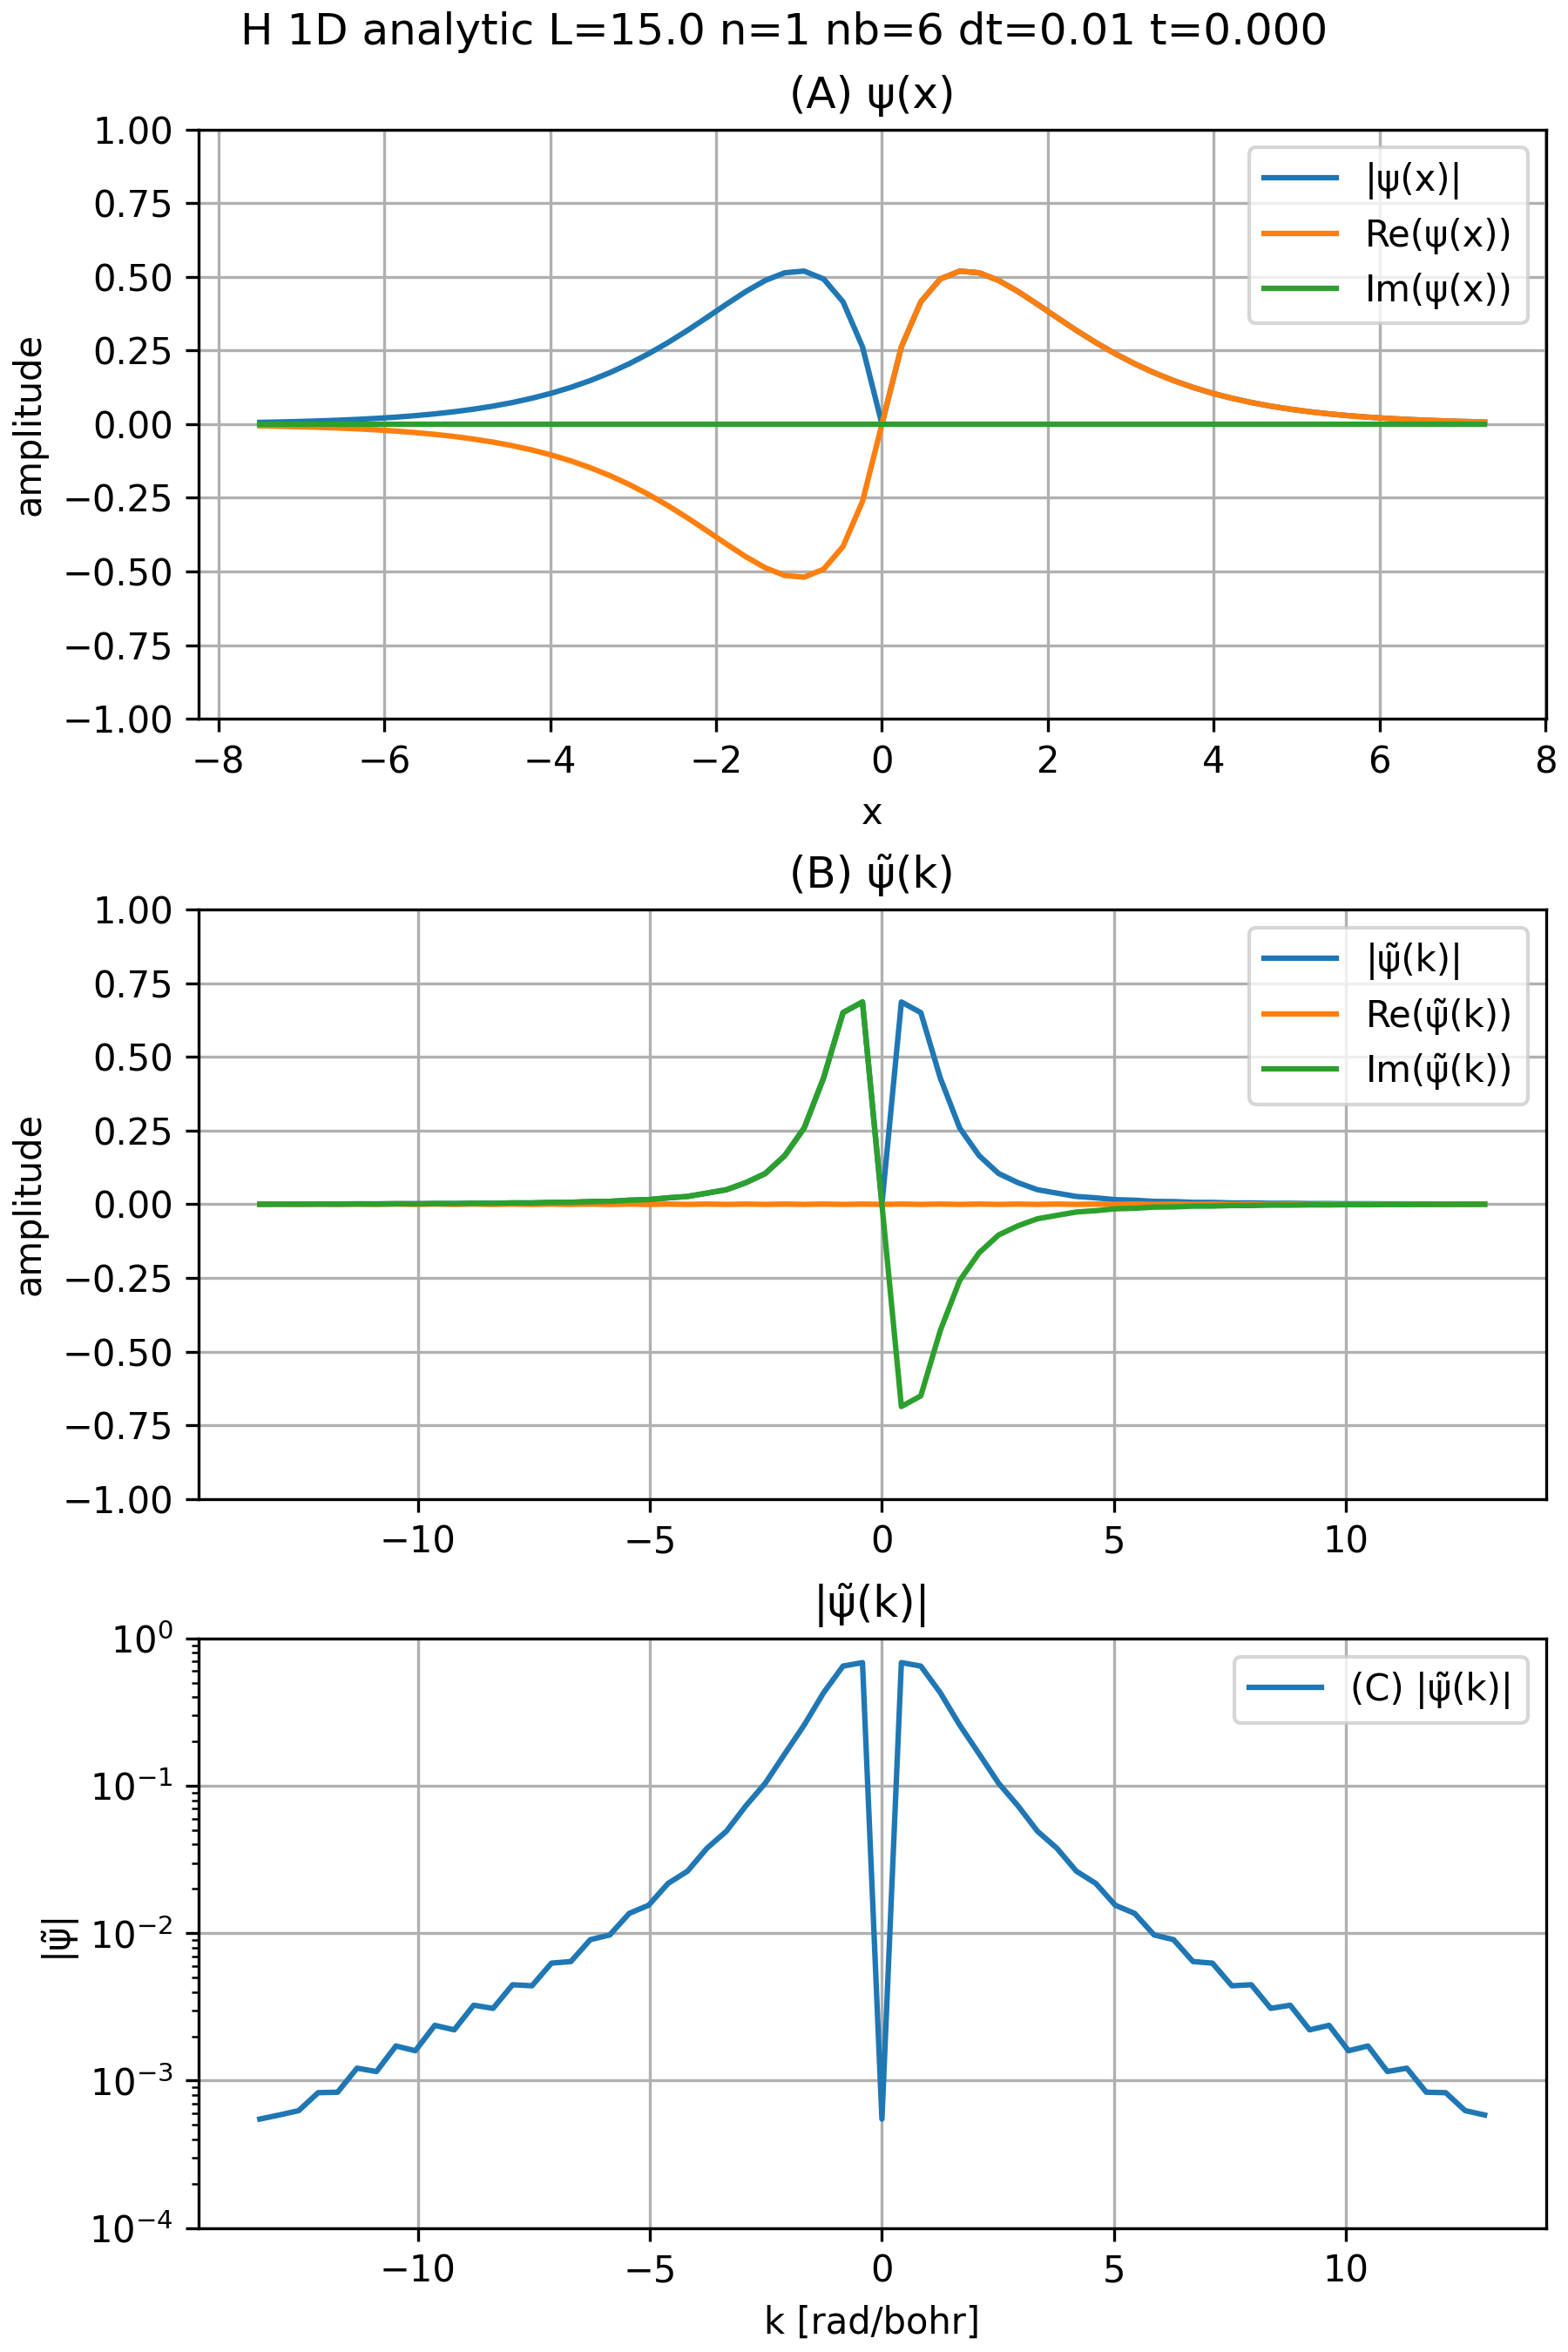
\includegraphics[width=0.6\textwidth]{paper2025_figs/analytic1D/t_00.000.png}
    \caption{Example of the 1D model wave function $\PsiOneD_1$}
    \label{fig:initial-wavefunction-1d}
    \begin{flushleft}\small

        Values of $\PsiOneD_1$ (Eq. \eqref{eq:psi1D1-wave-function}) at 6-bit
        resolution. (A) shows the wave function amplitude in real-space. (B)
        shows the wave function amplitude in k-space. (C) is a logarithmic scale
        representation of the amplitude in k-space.
    \end{flushleft}
\end{figure}

For the 2D model, we use the analytical solution by Parfitt
\cite{Parfitt2002.10.1063/1.1503868}. This model restricts an electron moving
under the Coulomb potential, $-1/\sqrt{x^2+y^2}$ to a 2D plane. The wave function
has two quantum numbers, $n\in\{0,\ldots\}$ and $m\in\{-n,\ldots,0,\ldots,n\}$ as
parameters and is expressed as follows:

\begin{equation}
\psi_{n,\ m}^{\mathrm{2D}}(r,\ \theta)=
\sqrt{\frac{q_0^3(n-\abs{m})!}{\pi(n+\abs{m})!}}(2q_0r)^{\abs{m}}
e^{-q_0r}L_{n-\abs{m}}^{2\abs{m}}(2q_0r)e^{im\theta}
\end{equation}
where $q_0=1/(n+1/2)$. The energy eigenvalue is given using the quantum number $n$ as:
\begin{equation}
E_n^{\mathrm{2D}}=-\frac{1}{2(n+1/2)^2}
\end{equation}
For evaluation, we use the ground state $\psi_{0,0}^{\mathrm{2D}}$ and the excited states $\psi_{1,0}^{\mathrm{2D}}$ and $\psi_{1,1}^{\mathrm{2D}}$. Their respective wave functions and eigenvalues are as follows:
\begin{align}
\psi_{0,0}^{\mathrm{2D}}(r,\theta)&=\sqrt{\frac{8}{\pi}}e^{-2r}
\label{eq:psi2D00-wave-function}\\
E_0^{\mathrm{2D}}&=-2
\label{eq:psi2D00-energy}\\
\psi_{1,0}^{\mathrm{2D}}(r,\theta)&=\sqrt{\frac{8}{27\pi}}(1-\frac{4}{3}r)e^{-\frac{2}{3}r} 
\label{eq:psi2D10-wave-function}\\
\psi_{1,1}^{\mathrm{2D}}(r,\theta)&=\frac{8}{9\sqrt{3\pi}}re^{-\frac{2}{3}r+i\theta}
\label{eq:psi2D11-wave-function}\\
E_1^{\mathrm{2D}}&=-\frac{2}{9}\simeq -0.2222
\label{eq:psi2D10-energy}
\end{align}

The position and wavenumber representations of these three states are shown in
Fig. \ref{fig:initial-wavefunction-2d-00_10}(a), Fig.
\ref{fig:initial-wavefunction-2d-00_10}(b), and
Fig. \ref{subfig:initial-wavefunction-2d-1-1}, respectively.

\begin{figure}
    \centering
    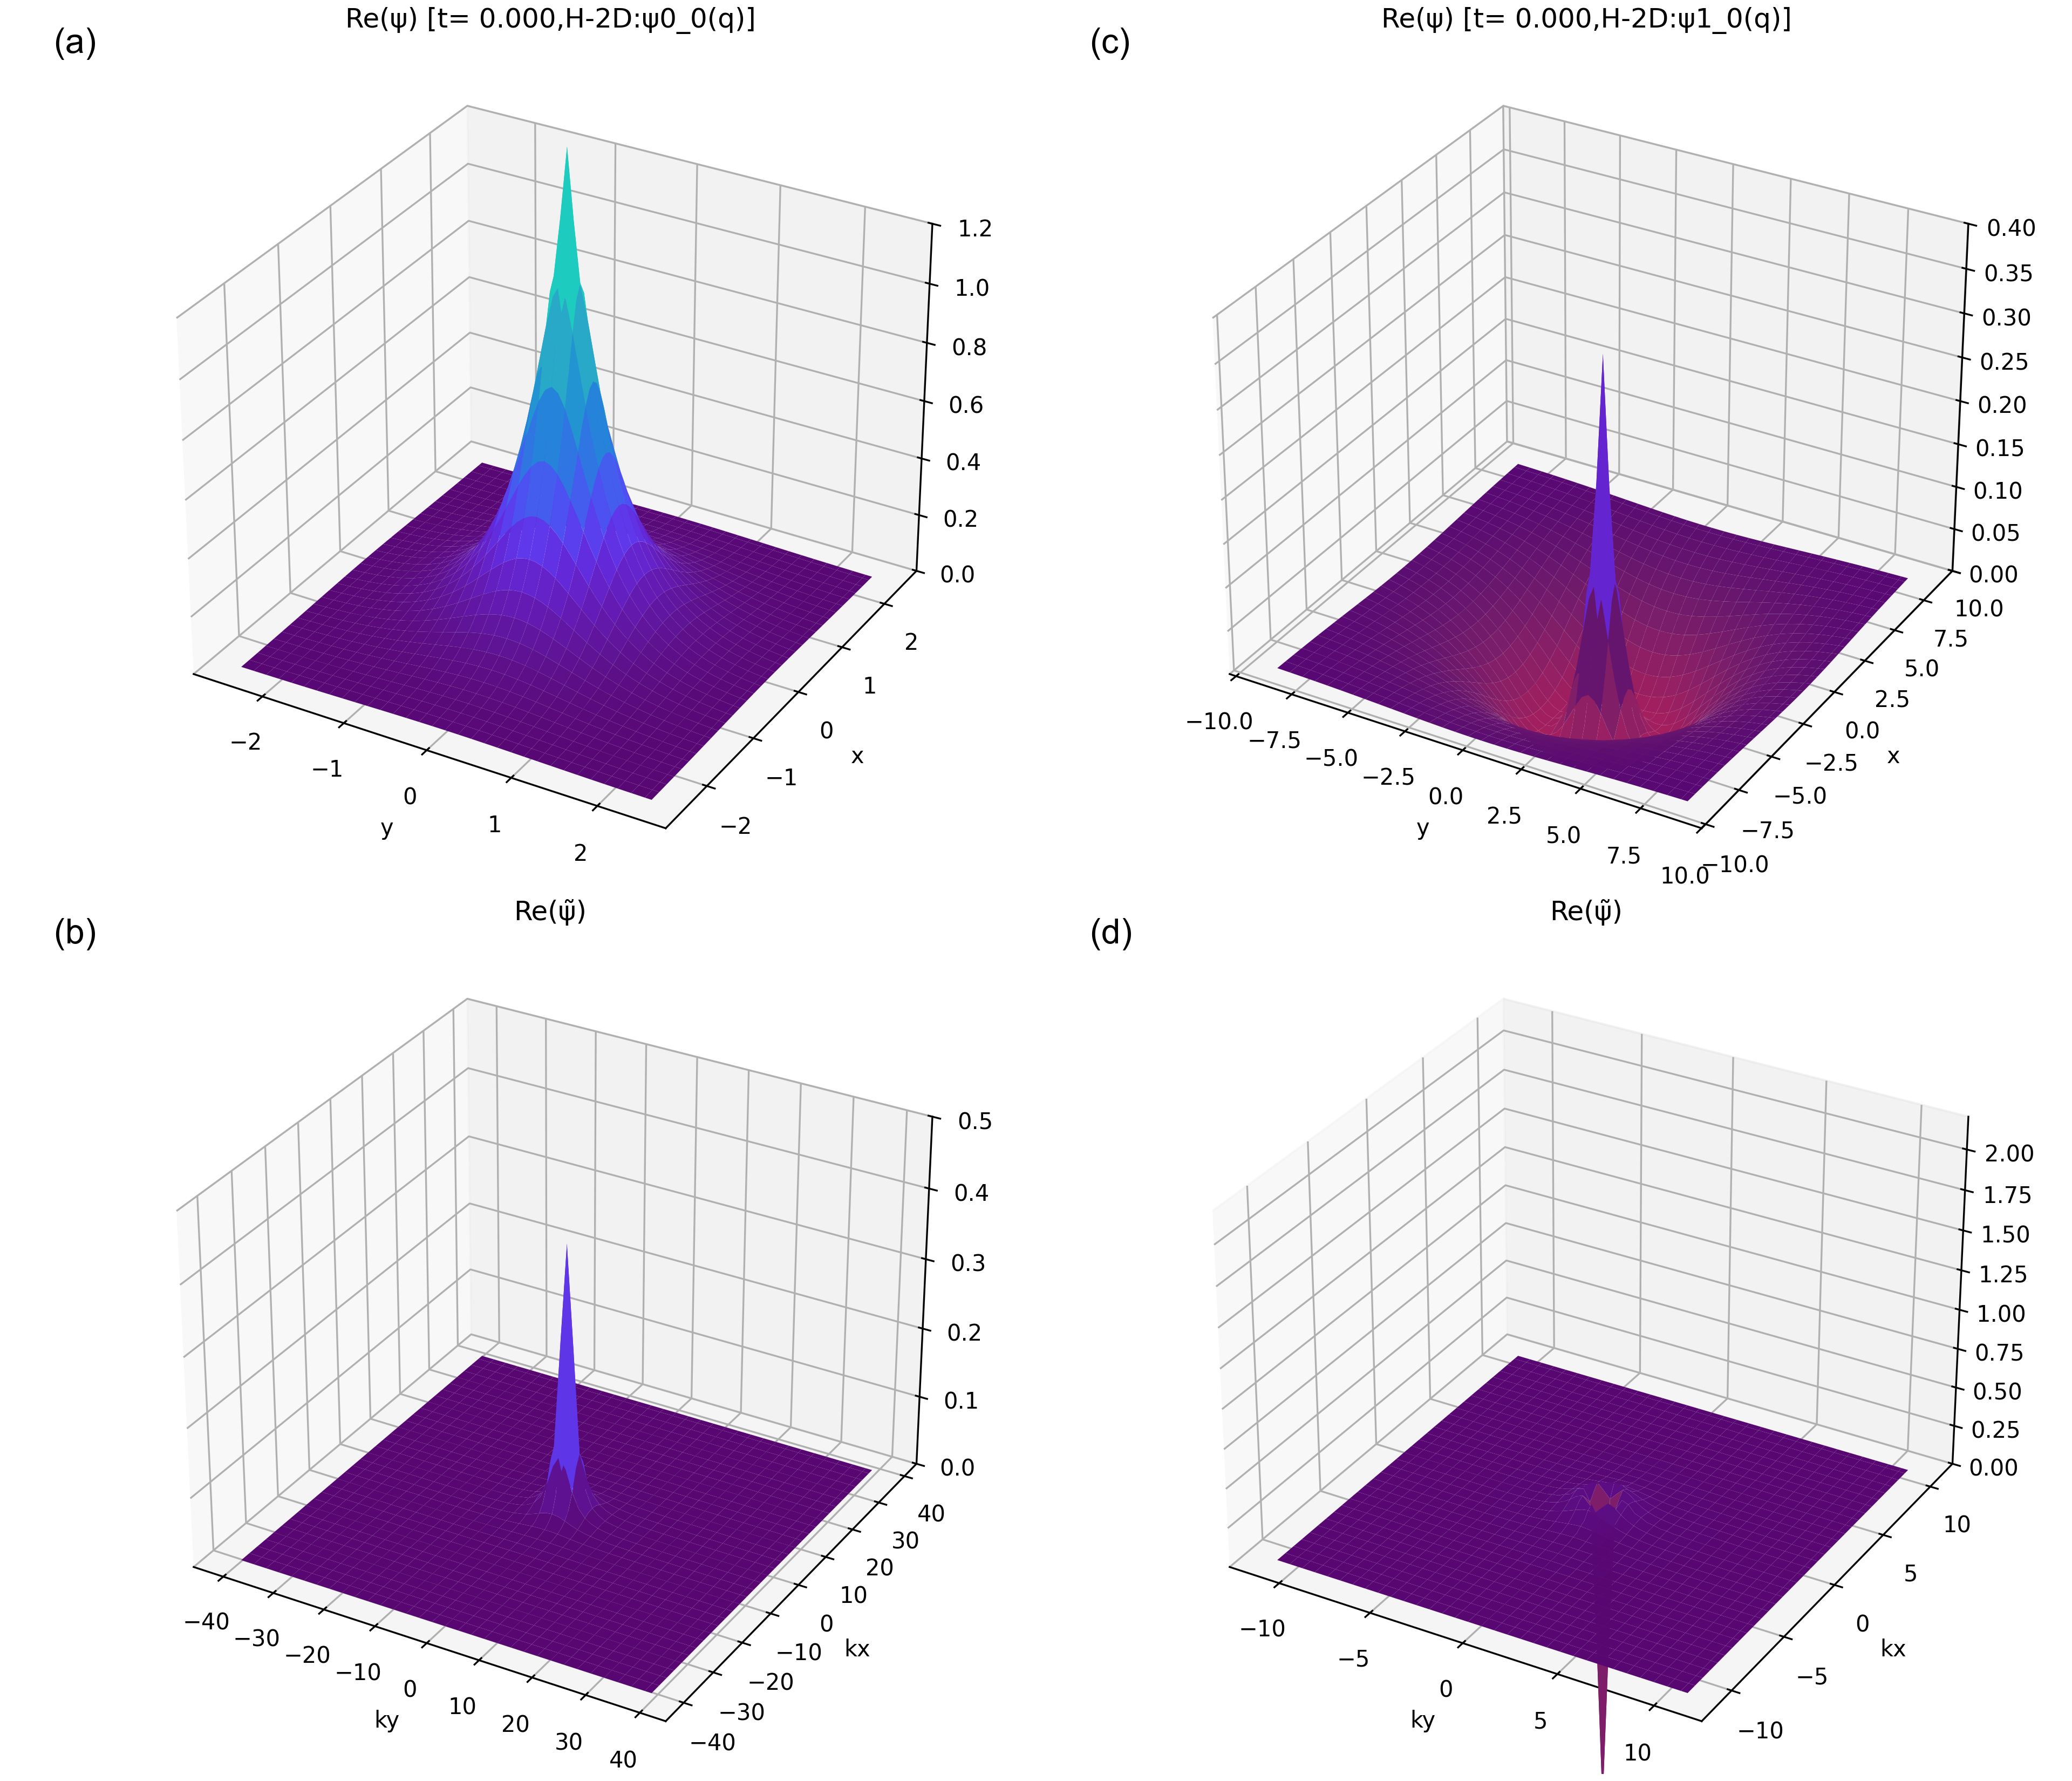
\includegraphics[width=1\columnwidth]{paper2025_figs/classic2D/initial-wavefunction-2d-00_10.png}
    \caption{Wave functions $\PsiTwoD_{0,0}$ and $\PsiTwoD_{1,0}$}
    \label{fig:initial-wavefunction-2d-00_10}
    \begin{flushleft}\small 

        (a) Real part of the wave function for the ground state $\PsiTwoD_{0,0}$
        with principal quantum number $n=0$ and azimuthal quantum number $m=0$
        (Eq. \eqref{eq:psi2D00-wave-function}). (b) Real part of the Fourier
        transform of the wave function for the same state. (c) Real part of the
        wave function for the excited state $\PsiTwoD_{1,0}$ with $n=1, m=0$
        (Eq. \eqref{eq:psi2D10-wave-function}). (d) Real part of the Fourier
        transform of the wave function for the same state. Both (a) and (c) have
        non-zero wave function values at the origin.
    \end{flushleft}
\end{figure}

\begin{figure}
    \centering
    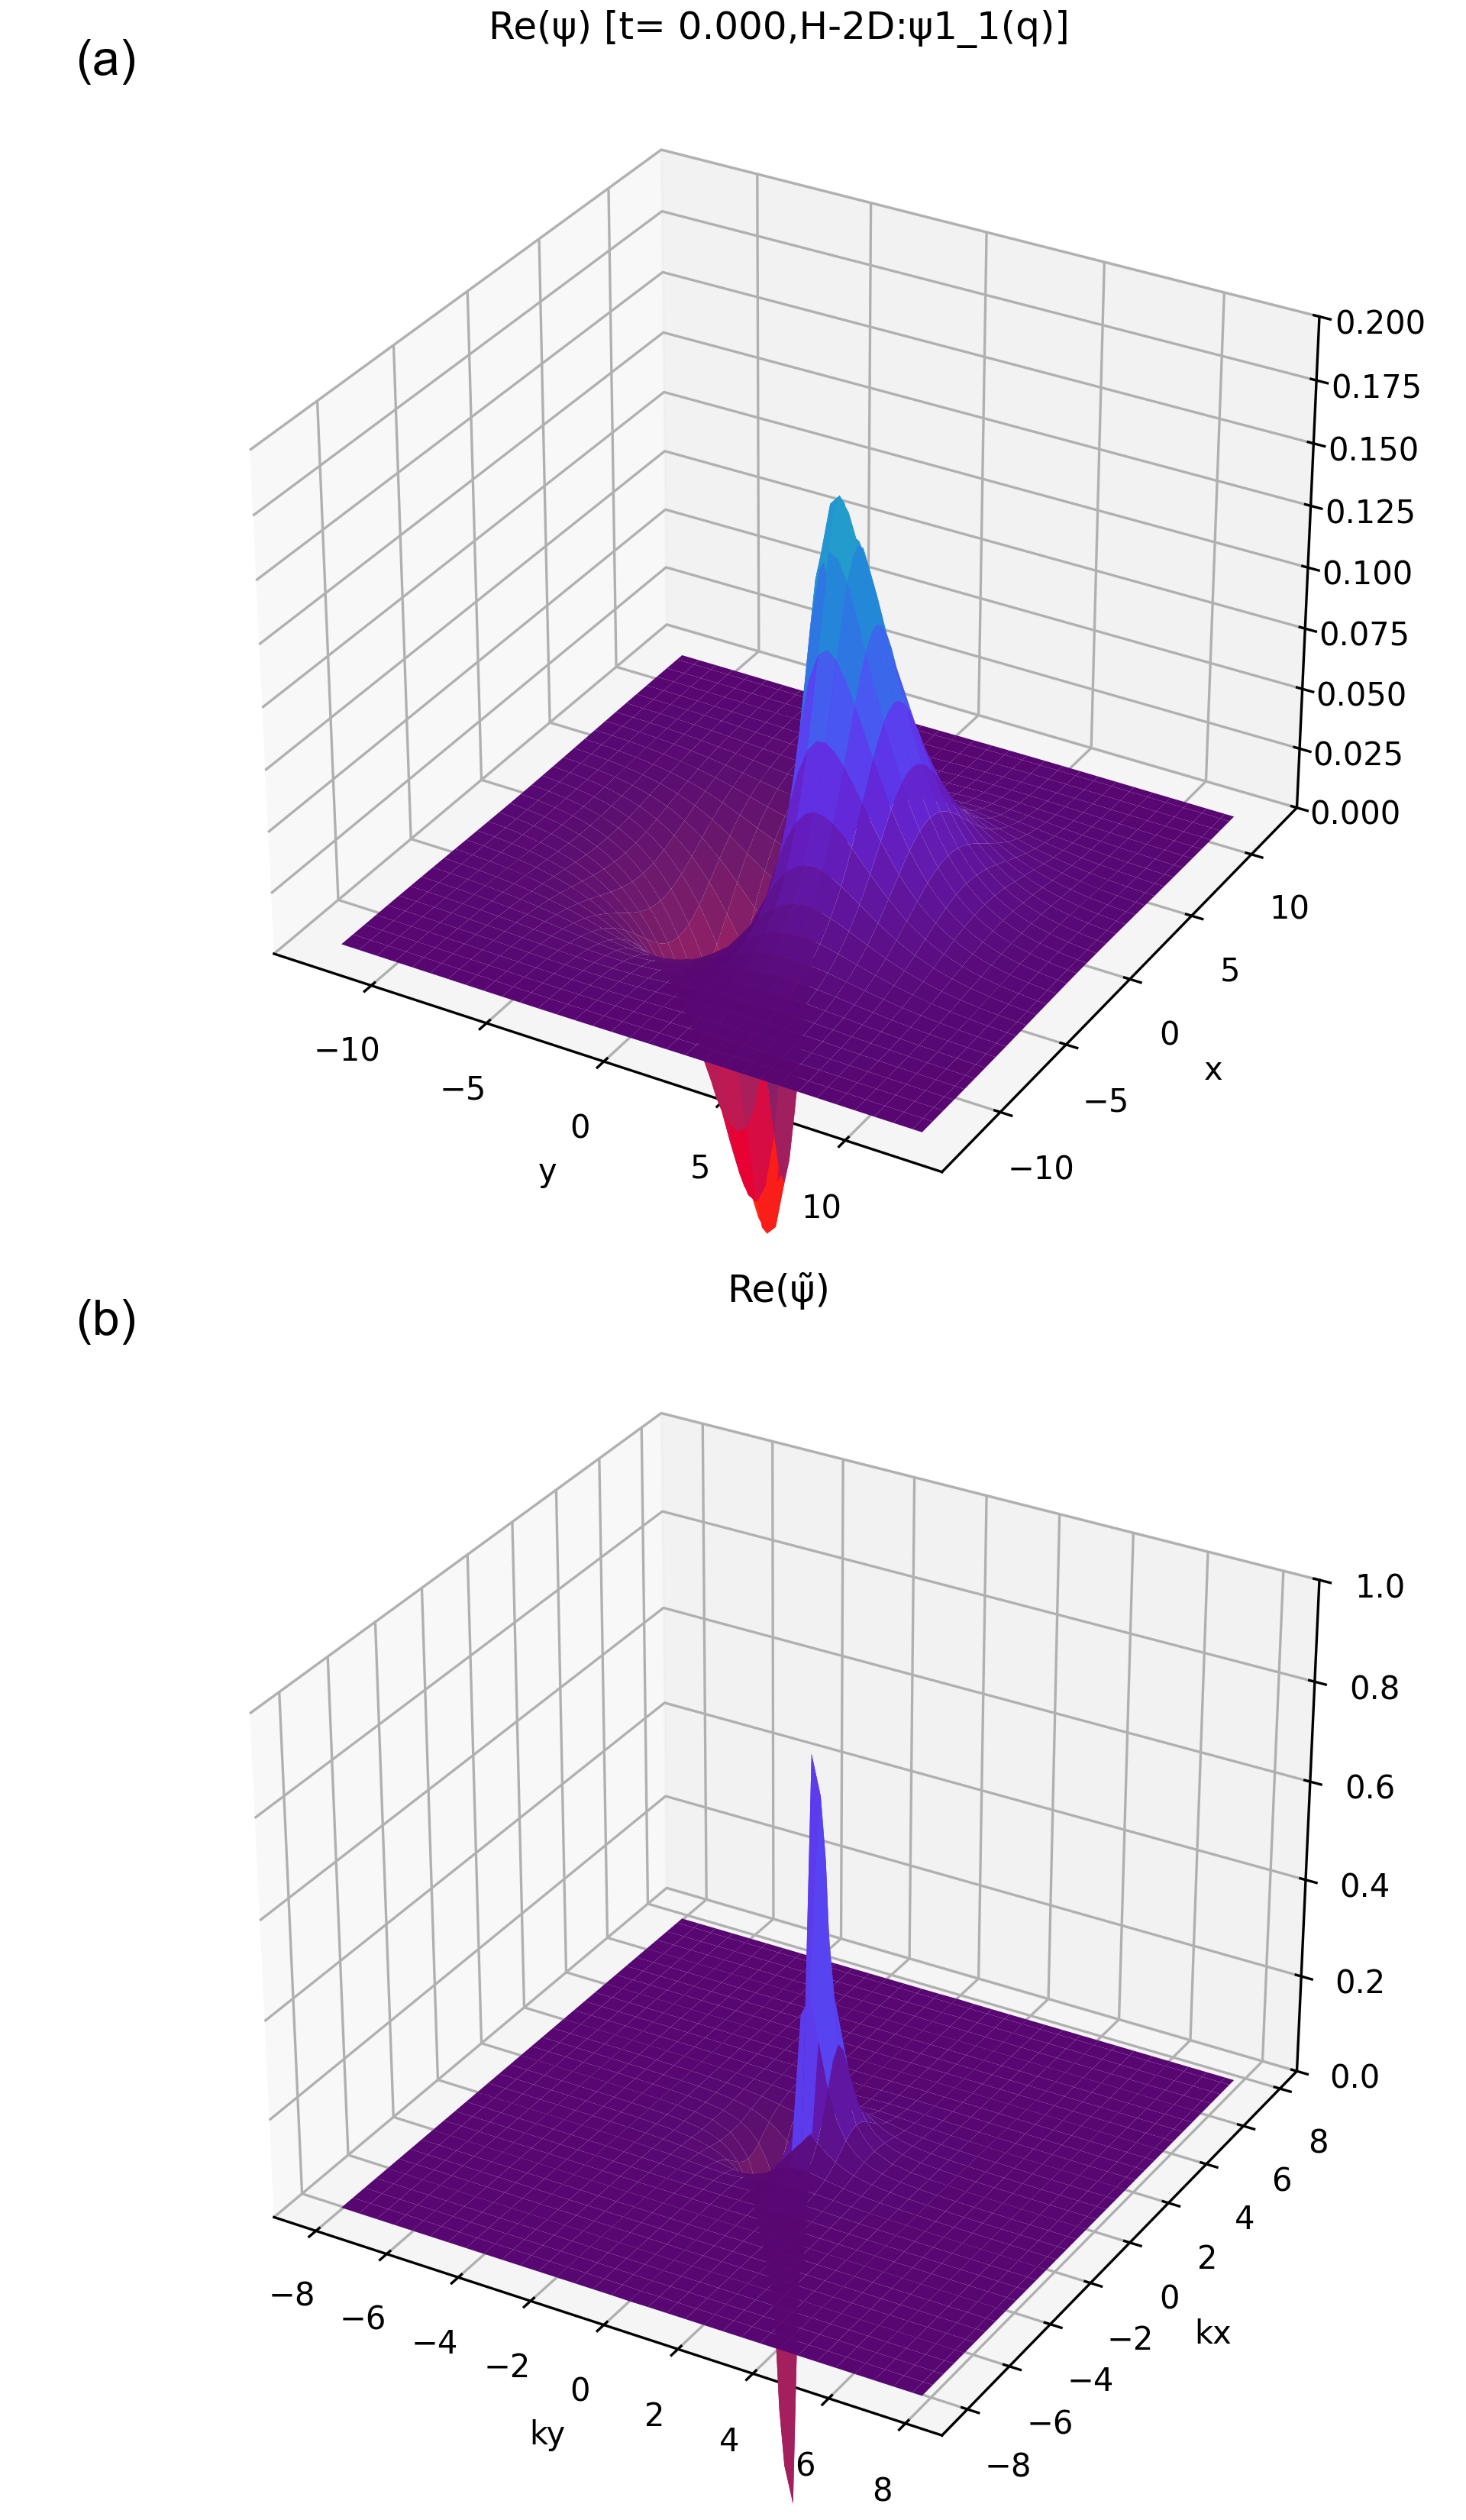
\includegraphics[width=0.45\columnwidth]{paper2025_figs/classic2D/initial-wavefunction-2d-11.png}
    \caption{Wave function $\PsiTwoD_{1,1}$}
    \label{subfig:initial-wavefunction-2d-1-1}
    \begin{flushleft}\small

        Excited state $\PsiTwoD_{1,1}$ with $n=1, m=1$ (Eq.
        \eqref{eq:psi2D11-wave-function}). (a) the real part of the wave
        function in real-space. (b) the real part of the wave function in
        k-space. The wave function value at the origin is zero.
    \end{flushleft}
\end{figure}

\clearpage
\subsubsection{Use of a Quantum Computer Emulator}
In this study, we execute quantum circuits using a quantum computer emulator on
a classical computer rather than actual quantum hardware. Specifically, we
utilized the emulator provided as part of the Qiskit SDK
\cite{website:qiskit-aer}.

The emulator holds the state vector of the qubits in the classical computer's
memory and executes quantum gate operations by expanding them as matrix
operations on the state vector. There are several methods for representing
the state. The simplest Statevector method holds the state vector of $N$ qubits
as an array of $2^N$ elements in memory. On the other hand, when quantum
entanglement between qubits is local, the Matrix Product State (MPS) method
\cite{Vidal2003.PhysRevLett.91.147902}, which represents the state as a tensor
network and significantly compresses memory usage, is effective and is supported
by the Qiskit emulator.

However, in the grid method based on first quantization, because the wave
function is mapped across the entire space, strong entanglement inherently
occurs among virtually all qubits (excluding ancilla qubits) during the time
evolution process. Therefore, we determined that the benefits of data
compression via the MPS method could not be obtained, and adopted the exact
Statevector method in this study.

Furthermore, as we premise future operation on FTQC (fault-tolerant quantum
computers), we do not consider hardware-specific noise in the circuit design,
and the emulator is operated as an ideal, noise-free quantum computer.

\subsubsection{Concurrent Use of a Classical Time Evolution Simulator}
To operate the simulator circuit on the emulator, the number of qubits and gates
must be kept within the range manageable by classical memory (generally fewer
than 30 qubits), which naturally restricts the range of specifiable simulation
parameters. Therefore, when evaluating parameter regimes that exceed the
emulator's execution limits, such as finer grid spacings, we concurrently used a
custom-implemented classical program designed to operate mathematically
equivalently to the quantum circuit. The combinations of parameters actually
executed on the emulator are shown in Table
\ref{tab:emulator-circuit-configurations} in Sec.
\ref{subsec:circuit-size-evaluation-results}.

\subsubsection{Computing Environment}
The computer hardware and software used for the simulation calculations are
shown in Table \ref{tab:computing-environment}.

\begin{table}[ht]
    \centering
    \caption{computing environment}
    \begin{tabular}{ll}
        item & description \\
        \hline
        CPU & AMD Ryzen 9 7950X 16 Core × 1 \\
        Memory & 128GB \\
        GPU & NVIDIA GeForce RTX 4090 × 1 \\
        OS & Ubuntu 22.04.4 LTS \\
        Quantum SDK & Qiskit 1.4.0, qiskit-aer-gpu 0.15.1 \\
        Quantum Chemistry Simulator Software & Chemical Reaction Simulator Q (crsQ) \cite{website:crsq}
    \end{tabular}
    \label{tab:computing-environment}
\end{table}

\subsection{Design of Potential Calculation Circuits that fits on an Emulator}
\label{subsec:design-of-potential-calculation}
This section describes the design of a circuit configuration executable on an
emulator, which is the first of the three main challenges addressed in this
study. To realize a simulation that fits within an emulator with a limited
number of qubits, in addition to simplifying the computational model itself
(restricting it to 1D and 2D and fixing the nucleus, as described in Sec.
\ref{subsec:simulator-model}), significant simplification of the quantum circuit
is essential. This section focuses particularly on the implementation techniques
for the Coulomb potential calculation circuit, which accounts for the majority
of the circuit size.

A standard approach to quantum circuit design in quantum chemistry simulation
starts with the size of the target molecular model and the amount of acceptable
error to estimate the required number of qubits and gates. In contrast, this
study takes a reversed approach: starting with the number of qubits available
(or emulatable) to the circuit and exploring/determining a circuit configuration
that can operate under that constraint. Therefore, we adopt methods that can
minimize the constant overhead (especially the number of ancilla qubits) to the
utmost limit for small-scale models, even if they are unsuitable for large-scale
models from an asymptotic scaling perspective.

In the fundamental approach based on the Suzuki-Trotter decomposition in first
quantization, the target space is divided into equally spaced grids, grid
indices are mapped to qubit registers, and arithmetic circuits are used to
calculate the Coulomb potential \cite{Zalka-rspa.1998.0162}. Because the number
of qubits and gates in this method scales polynomially with the number of
particles, it is exponentially more efficient than algorithms on classical
computers. However, while asymptotically efficient, the constant coefficients
for the number of ancilla qubits and gates associated with arithmetic operations
are by no means small.

In previous studies of first-quantization simulations, methods combining QROM
(Quantum Read-Only Memory) and the Newton-Raphson method to approximate the
potential have been proposed to avoid computationally expensive square root and
division operations \cite{Rubin2024.pnas.2317772121,
Babbush_2018b.PhysRevX.8.041015, Sanders2020.PRXQuantum.1.020312}. While this
approach is extremely effective for reducing gate depth, the structure of the
QROM circuit requires a large number of ancilla qubits proportional to the
number of output bits. Because the emulator environment (and early FTQC devices)
assumed in this study faces strict limits on the number of available qubits, we
opt against this method. Instead, we adopt and evaluate qubit-efficient
implementation techniques using arithmetic circuits and UCRZ circuits, as
described in the following subsections.

\subsubsection{Implementation Using Arithmetic Gates}
\label{subsubsec:implementation-using-arithmetic-gates}

The fundamental method for the Coulomb potential calculation circuit is based on
arithmetic circuits \cite{Zalka-rspa.1998.0162}.

\begin{figure}[ht]
    \centering
    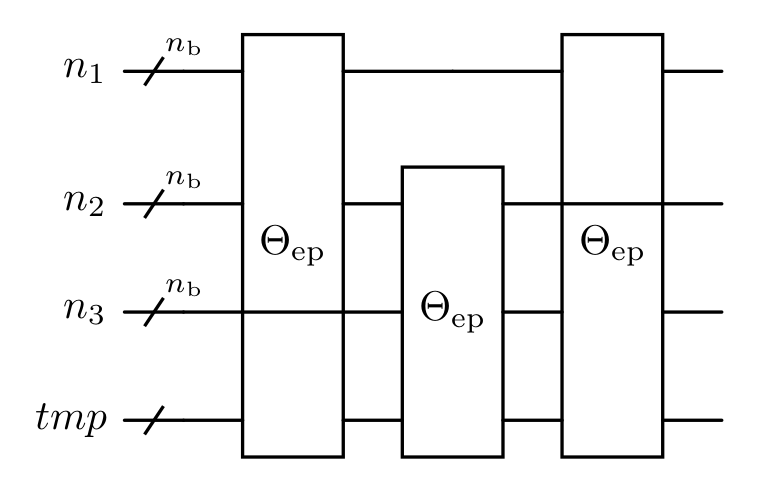
\includegraphics[width=0.4\columnwidth]{paper2025_figs/quantikz/arith.png}

    \caption{Example of the Coulomb potential term circuit $\Thetaep$ in a 3-electron system}
    \label{fig:theta-ep-multi-electron}
    \begin{flushleft}\small

        $n_1, n_2, n_3$ are registers corresponding to the discretized
        coordinates of electrons 1, 2, and 3, respectively, each consisting of
        $\nb$ bits. The slash on the qubit line indicates a register consisting
        of multiple qubits rather than a single qubit. $tmp$ is an ancilla qubit
        register. The Coulomb potential calculation circuit $\Thetaep$ must be
        applied to each of the three electron pairs (1,2), (2,3), and (1,3), but
        a single ancilla qubit register can be reused if prepared once. A qubit
        line passing straight through a $\Thetaep$ circuit box indicates that
        the qubit is not manipulated during that circuit operation.
    \end{flushleft}
\end{figure}

This circuit requires ancilla qubits on the order of $O(\nb)$ to hold
intermediate calculation values. When handling a system with multiple particles,
calculation circuits are required for each particle pair; however, a single set
of ancilla qubits can be initialized and repeatedly used between calculations
for different pairs. Thus, as shown in Fig. \ref{fig:theta-ep-multi-electron},
the total number of required ancilla qubits remains constant even as the number
of particles increases. Consequently, the number of ancilla qubits itself is
rarely viewed as problematic in evaluations of asymptotic scaling. Nevertheless,
in small-scale emulator environments where only a few dozen qubits are
available, even this constant number of ancilla qubits occupies an extremely
large proportion of the entire circuit, becoming a factor that severely limits
the simulatable model size.

\clearpage

\subsubsection{Implementation Using UCRZ Gates}
\label{subsubsec:implementation-using-ucrz-gates}

In this study, we focused on the Uniformly Controlled Rotation (UCR) circuit
\cite{Mottonen2004.PhysRevLett.93.130502}, which has an effect similar to QROM,
as a means to drastically reduce the number of ancilla qubits, which is fatal
for small-scale models.

A UCRZ circuit, a variation of the UCR circuit, rotates the target qubit around
the Z-axis depending on the state of an input register. Because the potential
term of the time evolution operator is defined exactly as a phase rotation for
each state, the operation of the UCRZ circuit can be directly utilized as the
Coulomb potential application process. This makes it possible to pre-compute the
inter-particle distance and its inverse square root and embed them into the
rotation angle parameters of a single UCRZ circuit, thereby reducing the large
number of ancilla qubits---essential in arithmetic circuits---down to just one
target qubit.

However, since the number of gates in a UCRZ circuit increases exponentially
with the number of bits in the input register, its application to large-scale
registers is impractical. Still, in verifying small-scale models where the total
number of qubits is strictly limited, it serves as an extremely effective means
to increase the number of qubits available for the coordinate register by
reducing the number of ancilla qubits. By adopting this UCRZ circuit, we
achieved a complete quantum circuit simulation of a 2D model on an emulator in
this study.

The action of a UCR circuit is generally described as follows:
\begin{equation}
    \ket{b}\ket{t} \mapsto \ket{b} R_{\mathrm{a}}(\theta_{\mathrm{b}})\ket{t}
\end{equation}

\begin{figure}[ht]
    \centering
    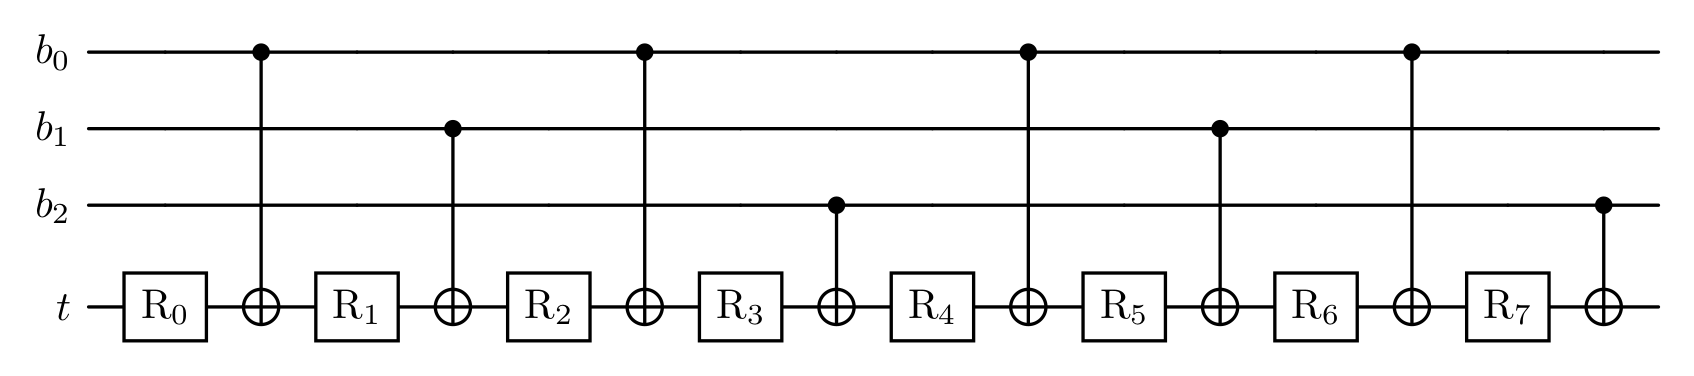
\includegraphics[width=0.8\columnwidth]{paper2025_figs/quantikz/ucrz.png}
    \caption{Example of a 3-bit input UCRZ circuit}
    \label{fig:ucrz-n3}
    \begin{flushleft}\small

    For a 3-bit input register $b_2b_1b_0$, there are 8 possible states, and 8
    Rz gates act on the target qubit $t$ to provide the corresponding phase
    rotation for each state. $\mathrm{R}_k$ denotes $\mathrm{Rz}(\theta_k)$. CX
    (C-NOT) gates placed before and after each Rz gate invert the sign of the Rz
    gate's rotation depending on the bit string of the input register. The map
    between the desired output angle $\alpha_b$ for input $b=b_2b_1b_0$ and the
    rotation angle $\theta_k$ is simplified by treating the bit string
    $b_2b_1b_0$ as a binary number in gray code.

\end{flushleft}
\end{figure}

An $n$-bit input UCRZ circuit has a structure where CX gates and Rz gates
applied to the target qubit are arranged alternately $2^n$ times. An example of
a 3-bit input UCRZ circuit is shown in Fig. \ref{fig:ucrz-n3}
\cite{Mottonen2004.PhysRevLett.93.130502}.

The $k$-th Rz gate $\mathrm{R}_k$ rotates the phase by a predetermined angle
$\theta_k$. In the absence of CX gates causing parity inversion, the overall
rotation angle of the circuit is simply the sum of $\theta_k$. However, when a
target CX gate is activated (control bit is 1), the relationship
$\mathrm{X}\mathrm{R_z}(\theta)\mathrm{X} = \mathrm{R_z}(-\theta)$ is applied to
the Rz gates flanked by that CX gate, reversing the sign of the rotation angle.
This is represented in matrix form as follows:

\begin{equation}
    \mathrm{X}\mathrm{R_z}(\theta)\mathrm{X} = 
    \begin{pmatrix} 0 & 1 \\ 1 & 0 \end{pmatrix}
    \begin{pmatrix} e^{-i\theta/2} & 0 \\ 0 & e^{i\theta/2} \end{pmatrix}
    \begin{pmatrix} 0 & 1 \\ 1 & 0 \end{pmatrix}
    = \begin{pmatrix} e^{i\theta/2} & 0 \\ 0 & e^{-i\theta/2} \end{pmatrix}
    = \mathrm{R_z}(-\theta)
\end{equation}

Because each bit of the input register $b$ is connected to the control bit of
the CX gates, the combination of Rz gates whose signs are inverted changes
depending on the value of the state $\ket{b}$. Consequently, the total phase
rotation angle $\alpha_b$ acting on the state $\ket{b}$ is as follows:

\begin{equation}
    \alpha_b = \sum_{k}{(-1)^{f_k(b)}\theta_k}
\end{equation}

Here, $f_k(b)$ is the parity (0 or 1) determined by the state $b$ and the gate
index $k$. Since the transformation from the vector of $\theta_k$ to the vector
of $\alpha_b$ is an invertible linear transformation, once all the desired phase
rotation angles $\alpha_b$ are given, the rotation angle $\theta_k$ for each
hardware gate can be uniquely determined by calculating the inverse matrix.

In our application to the Coulomb potential term circuit, we set the qubits
corresponding to the spatial coordinates of the particle as the input register
of the UCRZ circuit. Based on the potential energy $\Hep(\deltar\bm{\chi}_b)$ at
the discretized coordinate $\bm{\chi}_b$ corresponding to state $\ket{b}$, we
specify the phase rotation angle $\alpha_b$ to be applied as follows:

\begin{equation}
\alpha_b = -\frac{\Hep(\deltar\bm{\chi}_b)\deltat}{\hbar}
\end{equation}

By constructing a UCRZ circuit using the $\theta_k$ obtained through inverse
transformation of these values, the potential energy term $\Thetaep$ of the time
evolution operator can be strictly realized without consuming any ancilla
qubits.

\subsection{Regularization methods for the Coulomb Potential}
\label{subsec:coulomb-potential-handling}
When calculating the Coulomb potential via quantum circuits in
first-quantization-based simulations, avoiding divergence at the singularity
(pole, $r=0$) is an inevitable challenge. Because the potential energy term of
the time evolution calculation advances the phase of the wave function by an
angle proportional to the potential energy $-1/r$ at each grid point, the value
diverges at the point where the coordinates of the nucleus and the electron
coincide.

Approaches to address this divergence are broadly classified into the following
two categories: (a) methods that introduce approximation or regularization into
the potential function itself to prevent divergence even when the inter-particle
distance becomes zero; and (b) methods that mathematically prevent the distance
between the electron and the nucleus from strictly reaching zero by shifting the
coordinate of nuclei by a half-grid spacing ($\deltar/2$)
\cite{Chan2023.sciadv.abo7484}.

While method (b) is straightforward, the steep gradient of the potential near
the pole tends to increase the Suzuki-Trotter decomposition error, prompting
Chan et al. to apply post-processing corrections to their computational results.
In contrast, to complete the process purely within the framework of quantum
circuit computation, this study adopts approach (a), which approximates and
regularizes the potential function.

In this section, we examine two techniques under approach (a). The first is the
local average potential proposed in this study, which uses an effective
representative value only at the singularity. The second is the soft-core
potential, which is widely used in existing research.

Note that a zero denominator in the Coulomb potential becomes a fatal
computational problem only when the wave function amplitude at the singularity
is non-zero. Among the analytical solutions handled in this paper, the odd
function solution $\PsiOneD_1$ of the 1D model and the states of the 2D model
where the azimuthal quantum number is $m \neq 0$ have zero amplitude at the
origin; thus, the potential value at the pole can be any finite value. However,
the $m=0$ solutions of the 2D model ($\Psi_{0,0}^{\mathrm{2D}}$ and
$\Psi_{1,0}^{\mathrm{2D}}$) have non-zero amplitudes at the origin, requiring a
rigorous prescription. Below, we derive appropriate regularization parameters
targeting the latter states (the derived values are also directly applicable to
the former states).

\subsubsection{Formulation of the Local Average Potential}

As the first method, we define the local average potential $\Hla$, which uses
the original Coulomb potential at coordinates other than the singularity and
replaces it with a finite value based on the effective distance $\reff$ only at
the singularity ($r=0$).

\begin{equation}
\Hla(r) = \begin{cases}
-\frac{1}{r} & (r>0) \\
-\frac{1}{\reff} & (r=0)
\end{cases}\label{eq:Halr}
\end{equation}

Because this function can be realized simply by a division denominator
replacement circuit based on the condition check for $r=0$, it has the advantage
of keeping the implementation cost low as a quantum circuit.

The appropriate value of the effective distance $\reff$ in this approximation can
be derived from geometric consistency as follows. In the potential term
calculation using the grid method, the value at the center coordinate of each
grid cell is taken as a representative value, and spatial integration is
approximated by multiplying it by the cell area. Although this representative
value diverges for the cell containing the singularity, the exact spatial
integral of the energy expectation value in a minute region near the singularity
itself possesses a finite value without diverging in spaces of two or more
dimensions. Therefore, we back-calculate $\reff$ so that the energy expectation
value obtained by integration within the minute region matches the result of the
approximate calculation using the representative value.

Specifically, we consider a minute circle centered on the pole with a diameter
equal to the grid spacing $\deltar$. Let $W_{n,m}$ be the expectation value of
the energy calculated using the true Coulomb potential for this circular region,
and let $W_{n,m}^\prime$ be the energy from the approximate calculation using
$-1/\reff$ as the representative value at the pole.

\begin{align}
    W_{n,m}&=\int_{\theta=0}^{2\pi}d\theta\int_{r=0}^{\deltar/2}
    \Hep(r)\abs{\PsiTwoD_{n,m}(r)}^2r dr\\
    W_{n,m}^\prime&=\pi\left(\frac{\deltar}{2}\right)^2
    \Hla(0)\PsiTwoD_{n,m}(0) \notag \\
    &=-\frac{\pi\deltar^2}{4\reffnm{n,m}}
    \sqrt{\frac{q_0^3(n-\abs{m})!}{\pi(n+\abs{m})!}}
    L_{n-\abs{m}}^{2\abs{m}}(0)
\end{align}

Solving for states $(n,m)=(0,0)$ and $(1,0)$ so that these values match
($W_{n,m}=W_{n,m}^\prime$) yields the following:

\begin{align}
    \reffnm{0,0} &=\frac{q_0\deltar^2}{4(-e^{-q_0\deltar}+1)}
    \simeq \frac{q_0\deltar^2}{4(-1+q_0\deltar+1)}=\frac{\deltar}{4}
    \label{eq:delta-1-0-0}\\
    \reffnm{1,0} &=\frac{q_0\deltar^2}{4((-1-q_0^2\deltar^2)e^{-q_0\deltar}+1)}
    \simeq \frac{q_0\deltar^2}{4((-1-q_0^2\deltar^2)(1-q_0\deltar)+1)}
    \simeq\frac{\deltar}{4}
    \label{eq:delta-1-1-0}
\end{align}

Here, the approximations are based on Taylor expansions assuming sufficient
spatial resolution ($q_0\deltar \ll 1$). The detailed derivation process is shown
in Appendix \ref{chap:appendix_derivation_derivation}.

As shown in Eqs. \eqref{eq:delta-1-0-0} and \eqref{eq:delta-1-1-0}, a universal
result of $\reff \approx \deltar/4$ is obtained regardless of the state. By
rewriting Eq. \eqref{eq:Halr} using this value, the local average potential is
determined as follows:

\begin{equation}
\HlaTwoD(r) = \begin{cases}
-\frac{1}{r} & (r>0) \\
-\frac{4}{\deltar} & (r=0)
\end{cases}
\label{eq:Hlar2d-fixed}
\end{equation}

A similar derivation cannot be applied to the 1D model. This is because, in the
1D case, the power of the distance in the volume element is zeroth order, which
fails to cancel out the divergence of the Coulomb potential. However, because
the solution for the 1D model has zero amplitude at the origin, assigning any
arbitrary finite potential value at the singularity does not affect the
calculated energy expectation value. Therefore, for the 1D model, we adopt a
value that leads to the simplest circuit implementation.

When a division by zero occurs in the division circuit employed in this study,
all bits of the output value become 1. In the circuit for the 1D model, where
the binary representation has a single digit for the integer part, this yields
the value $1.11111\dots_{(2)} \simeq 2_{(10)}$. From a practical standpoint,
choosing this value allows us to handle the singularity without requiring any
additional circuitry. Since the coordinates processed by the circuit are
discretized, the quotient $2_{(10)}$ corresponds to $2/\deltar$. This is
equivalent to setting $\reff = \deltar/2$. We adopt this value as the effective
distance for the 1D model. Accordingly, the local average potential for the 1D
model is defined as follows:

\begin{equation}
\HlaOneD(r) = \begin{cases}
-\frac{1}{r} & (r>0) \\
-\frac{2}{\deltar} & (r=0)
\end{cases}
\label{eq:Hlar1d-fixed}
\end{equation}

The evaluation results of the energy values obtained from the time evolution
simulations using these potentials are discussed in Sec.
\ref{subsubsec:local-average-potential-results}.

\subsubsection{Deciding the Offset of the Soft-core Potential}

The second method, the soft-core potential $\Hsc$, smoothly avoids divergence
throughout the space by introducing a small offset constant $\Delta$ into the
norm calculation used for the distance. It is defined as follows
\cite{Kivlichan_2017}:

\begin{equation}
\Hsc(r) = -\frac{1}{\sqrt{r^2+\Delta^2}}
\label{eq:Hsc2r}
\end{equation}

The soft-core potential is widely used in Hamiltonian simulations to model
physical systems where the direction of electron motion is constrained
\cite{Hall2009.PhysRevA.80.032507, Fernandez_1991,
LiChen2021.doi:10.1021/acs.jpca.1c00698}, as well as to prevent the divergence
of the Coulomb term \cite{Childs2022quantumsimulationof}.

The method for determining the parameter $\Delta$ varies depending on the
purpose of using the soft-core potential.

The first method applies when the soft-core potential is used to correct the
energy in reduced-dimensional models representing physical systems with
constrained motion. For instance, it is known that setting $\Delta=\sqrt{2}$ in
a 1D hydrogen atom model yields the ground-state energy eigenvalue of $-0.5\
\mathrm{a.u.}$, which is identical to that of the 3D hydrogen atom
\cite{Eberly1991.PhysRevA.44.5997}. In this context, however, the regularization
of the singularity is merely a byproduct; in a 3D model where no energy
correction is required, $\Delta=0$, leaving the divergence problem unresolved.

The second method applies when the soft-core potential is used purely to avoid
the divergence at the singularity, which aligns with the focus of this study. To
the best of the authors' knowledge, there is no clearly established method in
the literature for determining $\Delta$ with a rational basis in this scenario.
Therefore, we propose setting $\Delta = \deltar/4$ so that the value of the
soft-core potential at the singularity ($r=0$) matches the analytically derived
local average potential discussed in the previous section. That is, the
soft-core potential used in our calculations is defined as follows:

\begin{equation}
\Hsc(r) = - \frac{1}{\sqrt{r^2+(\deltar/4)^2}}
\label{eq:Hsc2r-fixed}
\end{equation}

The evaluation results from time evolution simulations using this model are also
discussed in Sec. \ref{subsubsec:local-average-potential-results}, comparing
them with the results of the local average potential.

\subsection{Optimization of Simulation Parameters}
\label{subsec:optimization-of-simulation-parameters}

When executing Hamiltonian simulations, configuring the spatial resolution and
time step to keep calculation errors within a desired range is crucial, and
approaches to back-calculate the required number of qubits from a target
accuracy have been widely studied \cite{FEIT1982412, Kivlichan_2017,
Chan2023.sciadv.abo7484}. Conversely, under the premise that the number of
qubits is given (and strictly limited), this study focuses on the constraints
and tradeoff relationships that arise among each parameter, presenting a
parameter determination method to extract the best accuracy within limited
resources.

The results of time evolution simulations using the grid method and
Suzuki-Trotter decomposition employed in this study inherently include the
following errors:

\begin{equation}
\errtotal \leq \errspatial + \errtemporal
\label{eq:error-total-decomposition}
\end{equation}

Here, $\errtotal$ represents the total error, $\errspatial$ the spatial error,
and $\errtemporal$ the temporal error. These errors are further decomposed into
the following components:

\begin{align}
    \errspatial &\equiv \errdisc + \errcutoff \\
    \errtemporal &\equiv \erralias + \errtrotter
\end{align}
$\errdisc$ is the spatial discretization error (error due to approximating
continuous space with a grid), and $\errcutoff$ is the domain truncation error
(error due to the wave function extending beyond the rectangular simulation
domain). Additionally, $\erralias$ is the aliasing error (error caused by a
finite sampling frequency), and $\errtrotter$ is the Trotter error (error due to
the approximation of decomposing non-commuting operators).

To improve overall calculation accuracy, it is meaningless to drastically reduce
only a specific error component if other dominant errors remain. Therefore, it
is necessary to accurately grasp the tradeoff relationships among parameters and
reduce the bottleneck error terms in a balanced manner.

In this section, we discuss how to determine each parameter under the condition
that the total number of qubits is fixed. Because a tradeoff exists between
spatial parameters ($\deltar$ and $L$), we search for an optimal point that
minimizes the sum of both errors. On the other hand, while there is no tradeoff
for the temporal parameter ($\deltat$), a strict upper limit is required by the
sampling theorem and the analytical evaluation of the Trotter error, so we
determine a value that comprehensively satisfies these constraints.

\subsubsection{Criteria for Grid Spacing}
\label{subsec:criteria-for-grid-spacing}

In this study, the simulation target is a cubic domain applying periodic
boundary conditions, with a side length of $L=2^{\nb}\deltar$ (where $\nb$ is
the number of coordinate qubits for each dimension, and $\deltar$ is the grid
spacing). The center of this space is set as the origin of the coordinate
system, where the nucleus is placed.

Wave function components that fall outside the coordinate range $[-L/2, L/2)$
are forcibly cut off. Decreasing $\deltar$ reduces the spatial discretization
error $\errdisc$; however, because the number of qubits $\nb$ is fixed, the
domain size $L$ simultaneously shrinks, resulting in an increase in the
truncation error $\errcutoff$. Therefore, it is necessary to find the optimal
$\deltar$ where these two errors balance out and their sum is minimized.

Specifically, we define the value $S_1$ integrated over the square of the true
wave function within the simulation domain, and the value $S_2$ integrated
outside the domain, as follows:

\begin{align}
S_1 &= \int_{x,y,z=-L/2}^{L/2}\Psi(\bm{r})^{\ast}\Psi(\bm{r}) d\bm{r} \\
S_2 &= 1 - S_1
\end{align}

This is for the case of a 3D model, but the definitions for 1D and 2D models are
similarly given by integrating over the corresponding dimensions.

Meanwhile, let $S_d$ be the approximate calculation value on the discretized
coordinates corresponding to $S_1$:

\begin{equation}
S_d = \sum_{j}\abs{\Psi(\chij)}^2 \deltar^3
\end{equation}

At this time, each error factor can be estimated as follows:

\begin{align}
\errdisc &\simeq \abs{S_1 - S_d} \label{eq:err-disc-definition}\\
\errcutoff &\simeq S_2 \label{eq:err-cutoff-definition}
\end{align}

In other words, the $\deltar$ that minimizes the evaluation function $\abs{S_1 -
S_d} + S_2$ becomes the optimal grid spacing for a given number of qubits. The
numerical analysis results of this tradeoff using specific wave functions for
the 1D and 2D models are presented in Section
\ref{subsubsec:delta-r-selection-results}.

\subsubsection{Time Step Contraints from the Sampling Theorem}

\label{subsubsec:time-step-constraints-from-sampling-theorem}

The first condition that the time step $\deltat$ must satisfy is the avoidance
of aliasing errors derived from the properties of the Discrete Fourier Transform
(sampling theorem) \cite{FEIT1982412}. If one step of time evolution via the
Suzuki-Trotter decomposition is regarded as a sampling process, the amount of
phase rotation by the Hamiltonian must not exceed the Nyquist frequency; that
is, the maximum phase change per step must be less than a half-period ($\pi$).
This requires the following inequalities for the potential and kinetic energy
terms, respectively:

\begin{align}
\max_{\bm{r}}\abs{\Hep(\bm{r})\deltat/\hbar} < \pi \label{eq:nyqist-limit-by-hep}\\
\max_{\bm{k}}\abs{\Hek(\bm{k})\deltat/\hbar} < \pi \label{eq:nyqist-limit-by-hek}
\end{align}

First, we consider the case of the 1D model. When evaluating the inequality
\eqref{eq:nyqist-limit-by-hep} for the potential term, the true Coulomb
potential diverges at the pole. Therefore, we evaluate it using the
approximation formula for the local average potential ($\reff=\deltar/2$)
introduced in Sec. \ref{subsec:coulomb-potential-handling}:

\begin{equation}
\HlaOneD(r) = \begin{cases}
-\frac{1}{\abs{r}} & (r\neq0) \\
-\frac{2}{\deltar} & (r=0)
\end{cases}
\end{equation}

Because $\abs{\HlaOneD}$ is maximized at the pole ($r=0$), the condition becomes:

\begin{equation}
\max_{j}\abs{\Hep(\deltar\chij)\deltat/\hbar} = \frac{2\deltat}{\deltar\hbar}<\pi
\end{equation}

Solving this for $\deltat$ and using $L=2^{\nb}\deltar$ yields the upper limit $\deltatPmaxOneD$:

\begin{equation}
\deltat < \frac{\pi\deltar\hbar}{2}=\frac{L\pi\hbar}{2^{\nb+1}}\equiv\deltatPmaxOneD
 \label{eq:nyqist-limit-by-hep-final}
\end{equation}

Similarly, for the kinetic energy term inequality \eqref{eq:nyqist-limit-by-hek}:

\begin{equation}
\max_{\ell}\abs{\frac{\hbar^2(\kellx)^2}{2}\times\frac{\deltat}{\hbar}} < \pi
\label{eq:nyqist-limit-by-hek-maximum}
\end{equation}

The absolute value of the wavenumber $\kellx$ is maximized at the index $\ell =
-2^{\nb-1}$, where its value is $\kellx = (-2^{\nb-1})\times(2\pi/L)$.
Substituting this and solving for $\deltat$ gives the upper limit
$\deltatKmaxOneD$:

\begin{equation}
\deltat < \frac{L^2}{2^{2\nb-1}\hbar\pi}\equiv\deltatKmaxOneD
 \label{eq:nyqist-limit-by-hek-final}
\end{equation}

When converted to the number of Trotter divisions $\nT = T/\deltat$ for the
total simulation time $T$, the lower limits for the number of divisions are
determined as follows, respectively:

\begin{align}
    \nTpminOneD &= \frac{T}{\deltatPmaxOneD}=\frac{2^{\nb+1}T}{L\pi\hbar}
    \label{eq:nT-pmin-definition}\\
    \nTkminOneD &= \frac{T}{\deltatKmaxOneD}=\frac{2^{2\nb-1}\pi\hbar T}{L^2}
    \label{eq:nT-kmin-definition}
\end{align}

The number of time evolution divisions $\nT$ must be set to exceed both of these
lower limits.

Next, we evaluate the 2D model in the same manner. Regarding the potential term,
for both the local average potential $\HlaTwoD$ and the soft-core potential
$\HscTwoD$, the maximum value at the pole is equally determined by the parameter
$\reff=\Delta=\deltar/4$:

\begin{equation}
\max_{j}\abs{\HlaTwoD(\chij)\deltat/\hbar}
  = \max_{j}\abs{\HscTwoD(\chij)\deltat/\hbar}
  = \frac{4\deltat}{\deltar\hbar} < \pi
\end{equation}

From this, the potential-derived upper limit of $\deltat$ in 2D is obtained:

\begin{equation}
\deltat < \frac{\pi\deltar\hbar}{4}
        =\frac{L\pi\hbar}{2^{\nb+2}}
        \equiv\deltatPmaxTwoD
 \label{eq:nyqist-limit-by-hep-final-2D}
\end{equation}

For the kinetic energy term, the sum of the squares of the wave vectors
$(\kellx)^2+(\kelly)^2$ is maximized when $\kaplx=\kaply=-2^{\nb-1}$. Therefore,
substituting the maximum wavenumber into:
\begin{equation}
\max_{\ell}\abs{\frac{\hbar^2((\kellx)^2+(\kelly)^2)}{2}\times\frac{\deltat}{\hbar}} < \pi
\end{equation}
and rearranging yields the following upper limit:
\begin{equation}
\deltat < \frac{L^2}{2^{2\nb}\hbar\pi} \equiv\deltatKmaxTwoD
 \label{eq:nyqist-limit-by-hek-final-2D}
\end{equation}

The corresponding lower limits for the number of Trotter divisions are as follows:

\begin{align}
    \nTpminTwoD &= \frac{T}{\deltatPmaxTwoD}=\frac{2^{\nb+2}T}{L\pi\hbar} \\
    \nTkminTwoD &= \frac{T}{\deltatKmaxTwoD}=\frac{2^{2\nb}\pi\hbar T}{L^2}
\end{align}

\subsubsection{Time Step Constraints from Suzuki-Trotter Error}
\label{subsubsec:time-step-constraints-from-suzuki-trotter-error}

Another condition regarding the time step $\deltat$ arises from the requirement
of the approximation error $\errtrotter$ due to the Suzuki-Trotter
decomposition. Traditional error evaluations have relied on worst-case bounds
based on the operator norm $\| [H_1,H_2] \|$ of the commutators of the
Hamiltonian components, but this tends to overestimate actual simulation errors
\cite{Childs2021.PhysRevX.11.011020}. To perform a more rigorous and practical
error estimation, this study introduces the state-dependent Trotter error bound
proposed by Burgarth et al., which assumes a specific target wave function
\cite{Burgarth2024.PhysRevResearch.6.043155}.

While this does not directly provide a clear upper limit (threshold) for
$\deltat$ like the sampling theorem, using this evaluation formula allows us to
estimate an upper bound for the error given a set number of divisions $N$
(corresponding to $\nT$ in the notation of this paper). Assuming the initial
state is an eigenstate $\phi$ of the Hamiltonian $H_1+H_2$ with eigenvalue $h$,
the error $\xiN{1}(t;\phi)$ when evolved for time $t$ using the first-order
Suzuki-Trotter decomposition is bounded for an arbitrary constant
$g\in\mathbb{R}$ as follows \cite{Burgarth2024.PhysRevResearch.6.043155}:

\begin{equation}
    \xiN{1}(t;\phi)=\left\|\left[\SN{1}(t)-e^{-it(H_1+H_2)/\hbar}\right]\phi\right\|
    \leq\frac{t^2}{2N}\| \left(\|(H_1-g)^2\phi\|+\|(H_2-h+g)^2\phi\|\right)
    \label{eq:observed-trotter-error-1st}
\end{equation}

Here, $\SN{1}(t) = \left(e^{-i{tH}_1/N}e^{-itH_2/N}\right)^N$ is the first-order
time evolution operator. The minimum value of the right side of Eq.
\eqref{eq:observed-trotter-error-1st} is defined as $\BN{1}$:
\begin{equation}
\BN{1}(t;\phi)=\inf_{g\in\mathbb{R}}\frac{t^2}{2N}
    \left(\|(H_1-g)^2\phi\|+\|(H_2-h+g)^2\phi\|\right)
\label{eq:observed-trotter-error-bound-1st}
\end{equation}

This evaluation formula indicates that the order of the error is $O(t^2/N)$,
meaning the error decreases inversely proportional to the increase in the number
of divisions $N$ (however, it is pointed out that under conditions where $N$ is
extremely small or spatial resolution is high, this asymptotic behavior is
violated, becoming $O(t^2 N^{-1/4})$
\cite{Burgarth2024.PhysRevResearch.6.043155}).

Similarly, the error when using the second-order Suzuki-Trotter decomposition is
expressed by the following equation:

\begin{equation}
  \xiN{2}(t;\phi)\leq\frac{t^3}{N^2}\left(\frac{1}{24}\|H_1(g)^3\phi\| + \frac{1}{8}\|H_2(g)H_1(g)^2\phi\|
  +\frac{1}{12}\|H_2(g)^3\phi\|\right)
    \label{eq:observed-trotter-error-2nd}
\end{equation}
The minimum value $\BN{2}$ of the right side of this equation is given as follows:

\begin{equation}
\BN{2}(t;\phi)=\inf_{g\in\mathbb{R}}\frac{t^3}{N^2}
    \left(\frac{1}{24}\|H_1(g)^3\phi\| + \frac{1}{8}\|H_2(g)H_1(g)^2\phi\|
  +\frac{1}{12}\|H_2(g)^3\phi\|\right)
\label{eq:observed-trotter-error-bound-2nd}
\end{equation}

Here, $H_1(g) = H_1-g$ and $H_2(g) = H_2-h+g$.

In regions where the Trotter error $\errtrotter$ is dominant among the total
error (Eq. \eqref{eq:error-total-decomposition}), increasing the number of
divisions $N$ (i.e., $\nT$) can be expected to naturally improve the error
according to Eqs. \eqref{eq:observed-trotter-error-bound-1st} and
\eqref{eq:observed-trotter-error-bound-2nd}. Conversely, under conditions where
errors due to other factors such as spatial discretization are dominant,
increasing $N$ will not yield significant improvement in the overall error.

Combining the above, the absolute upper limit of the time step $\deltat$ is
dictated by the requirement of the sampling theorem (avoidance of aliasing), and
within that range, the number of divisions must be selected so that the Trotter
error falls within an acceptable limit. From the perspective of computational
cost (quantum circuit depth), it is desirable to adopt the largest possible
value for $\deltat$ (smallest $N$). Therefore, the strategy to determine the
optimal parameter in this method is to adopt the minimum number of divisions
within the range that contributes to the improvement of the overall error, while
assessing the balance with other error components.

\end{document}